% This is "sig-alternate.tex" V2.0 May 2012
% This file should be compiled with V2.5 of "sig-alternate.cls" May 2012
%
% This example file demonstrates the use of the 'sig-alternate.cls'
% V2.5 LaTeX2e document class file. It is for those submitting
% articles to ACM Conference Proceedings WHO DO NOT WISH TO
% STRICTLY ADHERE TO THE SIGS (PUBS-BOARD-ENDORSED) STYLE.
% The 'sig-alternate.cls' file will produce a similar-looking,
% albeit, 'tighter' paper resulting in, invariably, fewer pages.
%
% ----------------------------------------------------------------------------------------------------------------
% This .tex file (and associated .cls V2.5) produces:
%       1) The Permission Statement
%       2) The Conference (location) Info information
%       3) The Copyright Line with ACM data
%       4) NO page numbers
%
% as against the acm_proc_article-sp.cls file which
% DOES NOT produce 1) thru' 3) above.
%
% Using 'sig-alternate.cls' you have control, however, from within
% the source .tex file, over both the CopyrightYear
% (defaulted to 200X) and the ACM Copyright Data
% (defaulted to X-XXXXX-XX-X/XX/XX).
% e.g.
% \CopyrightYear{2007} will cause 2007 to appear in the copyright line.
% \crdata{0-12345-67-8/90/12} will cause 0-12345-67-8/90/12 to appear in the copyright line.
%
% ---------------------------------------------------------------------------------------------------------------
% This .tex source is an example which *does* use
% the .bib file (from which the .bbl file % is produced).
% REMEMBER HOWEVER: After having produced the .bbl file,
% and prior to final submission, you *NEED* to 'insert'
% your .bbl file into your source .tex file so as to provide
% ONE 'self-contained' source file.
%
% ================= IF YOU HAVE QUESTIONS =======================
% Questions regarding the SIGS styles, SIGS policies and
% procedures, Conferences etc. should be sent to
% Adrienne Griscti (griscti@acm.org)
%
% Technical questions _only_ to
% Gerald Murray (murray@hq.acm.org)
% ===============================================================
%
% For tracking purposes - this is V2.0 - May 2012

\documentclass{sig-alternate}
\usepackage{color}
\usepackage[usenames,dvipsnames]{xcolor}
\usepackage{url}

\newcommand{\TODO}[1]{{\color{red} TODO: #1}}
%\newcommand{\gametitle}{{\color{RoyalPurple} Dragon Architect}}
\newcommand{\gametitle}{{\emph{Dragon Architect}}}

\toappear{Submitted for review.}

\begin{document}
%
% --- Author Metadata here ---
%\conferenceinfo{Foundations of Digital Games (FDG)}{2015}
% \pdfinfo{
% /Title ()
% /Author (Aaron Bauer, Eric Butler, Zoran Popovic) 
% /Subject ()
% /Keywords ()
% }
%\CopyrightYear{2007} % Allows default copyright year (20XX) to be over-ridden - IF NEED BE.
%\crdata{0-12345-67-8/90/01}  % Allows default copyright data (0-89791-88-6/97/05) to be over-ridden - IF NEED BE.
% --- End of Author Metadata ---

\title{Dragon Architect: Guided Learning in a \\Creative Computer Science Sandbox Game}

\numberofauthors{1}
\author{Anonymized}

% \numberofauthors{1} 
% \author{
% \alignauthor
% Aaron Bauer, Eric Butler, Zoran Popovi\'c\\
%        \affaddr{Center for Game Science}\\
%        \affaddr{Computer Science \& Engineering}\\
%        \affaddr{University of Washington}\\
%        \affaddr{Seattle, WA 98195}
%        \email{\{awb, edbutler\}@cs.washington.edu}
% }

\maketitle
\begin{abstract}
Computer science is expanding into K12 education and numerous educational games and systems have been created to teach programming skills. We present \gametitle{}, an educational game built to explore under-researched questions in game-based learning and computer science education. Two research questions in computer science education we discuss are the teaching of abstract computational thinking skills and the effect of programming language semantics on novices. Because we seek to teach complex skills, we discuss research questions about learning in games. Open-ended games such as \emph{Minecraft} have proven valuable in an educational settings, but open-ended systems require outside instruction to be effective. We explore how to combine these games with more structured, linear learning experiences, and the impact of social environments on learning. We discuss how these research problems have informed the design of \gametitle{}, describe the design challenges encountered regarding those questions and player feedback, and survey current educational programming games and software.
\end{abstract}
% TODO replace macros in abstract so we don't accidentally paste them into form

% A category with the (minimum) three required fields
\category{K.3.2}{Computers and Education}{Computer and Information Science Education -- Computer science education}

\terms{Design, Human Factors}

\keywords{Game-based learning; computational thinking; programming education}

\section{Introduction}
% TODO move these citations somewhere
%Despite the proliferation of these systems, little work has investigated how to design the structure or content of such systems. There have been surveys of both the systems themselves~\cite{guzdial2004programming, kelleher2005lowering} and of research involving these systems~\cite{salleh2013analysis, backlund2013educational}. Researchers have enumerated desirable properties for such systems~\cite{repenning2010scalable} discussed their design~\cite{powers2006tools}.
%Comparative studies of effective ways to present computer science concepts in these systems, however, have been largely absent. A meta-analysis by Ke~\cite{ke2009qualitative} found that existing empirical research is fragmented and called for a more systematic approach.

The past few years have seen many efforts to broaden the reach of computer science education and make it available, and appealing, to more students in more places. As the expansion of computer science education, especially for primary and secondary-school students, gathers steam, we need more concrete data to guide the development of the educational systems and curricula. Many of the educational tools are programming environments for novice programmers, such as \emph{Scratch}~\cite{scratch} and Code.org's Hour of Code~\cite{codedotorg}. However, several areas of computers science education and game-based learning deserve of more research and investigation.

Two research questions in computer science education we hope to address are the teaching of \emph{computational thinking} and the effect of programming language semantics on novice programmers. Computational thinking is often discussed in the context of educational programming environments and there needs to be more research on how such systems can effectively teach these ideas. Important computational thinking skills include problem-solving strategies and meta-strategies, such as divide and conquer. We wish to explore how to directly teach such skills in the context of an educational game. As these skills will be learned and practiced in the context of programming, language design is a crucial part of the design of these systems. 

Exploring these questions lead to related research questions about effective methods of teaching in games. The structure of existing educational programming environments generally falls into one of two groups: (1) an open-ended setting with little to no direct guidance where players are intended to learn via exploration and from instructors or other members of the social community, or (2) a linear series of puzzles or exercises with substantial direct guidance, but little in the way of exploration of social interaction. Exploring the space in between these designs leads to many interesting questions and design challenges. An important method through which open-ended games can guide players in the social environment, and questions about how to foster such guidance in a programming game deserve special attention.

Our contributions are as follows: we survey research on teaching computational thinking in games and software systems and describe the open problems in that space, including how languages impact novices. We then survey and discuss related research problems in game-based learning. We a currently creating \gametitle{}, an educational game designed to investigate these questions. We describe design trade-offs and decisions in \gametitle{}, focusing on a few unsolved design obstacles: how to combine open-ended sandbox games with direct guidance, and how to encourage a social environment in a programming game. The focus of this paper is not on our game per se, but on the survey and discussion of open research problems in teaching computational thinking through games, and the design challenges and trade-offs encountered when building a game to tackle these problems.

\begin{figure*}[t!]
  \centering
  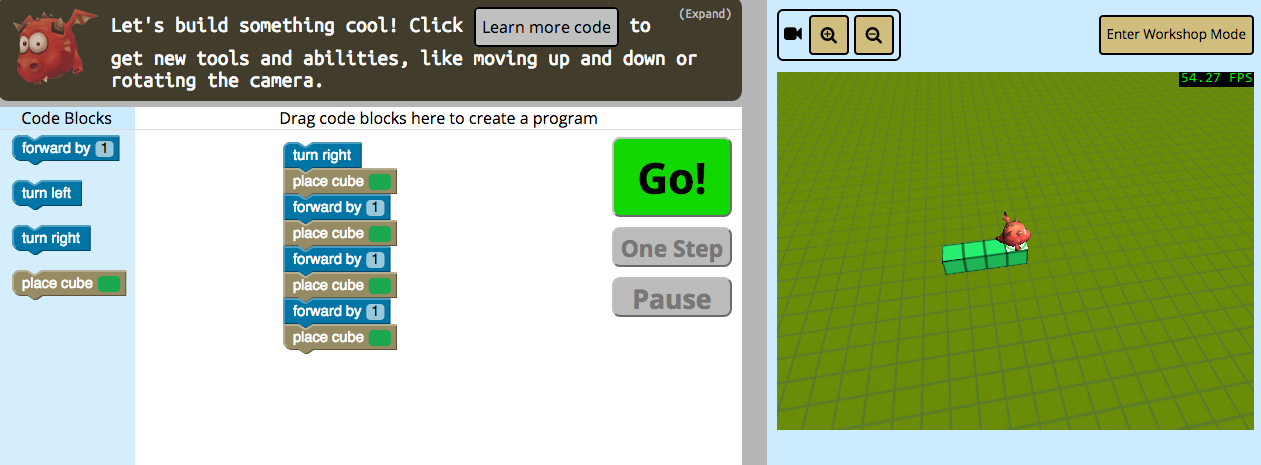
\includegraphics[width=\textwidth]{images/overall-example}
  \caption{The player assembles code for the dragon on the left side, and the dragon and world it inhabits are visualized on the right side. Only a few different code blocks are available to the player initially.}
  \label{fig:overall}
\end{figure*}

\section{Game Description}
Before we discuss open research problems and design challenges, we describe basic information about \gametitle{} to provide context for the discussion.
The game, which has been in development since spring 2014, can be played in a web browser.
Similar to other programming environments, the user interface is separated into two parts: an area where the player can assemble their code and a visualization of the 3D environment their code affects (see Figure~\ref{fig:overall}). 
The game uses the \emph{Unity} game engine~\cite{unity} for the 3D environment and the Blockly drag-and-drop programming library~\cite{blockly} for inputing code.

The visual language players use is a set of \emph{code blocks} that snap together to form programs. 
The player can move the dragon in three dimensions and have the dragon place and remove cubes of various colors. 
In addition to blocks that control the dragon directly, players can also make use of definite loops and procedures (see Figure~\ref{fig:toolbox}).
Given that syntax can be an obstacle for those new to programming~\cite{stefik2013syntax}, we chose to use a visual language as there is evidence visual languages are helpful to novices~\cite{whitley1997visual}.

As players progress through the game, they alternate between short sequences of puzzles with a specific goal and a specific set of available code blocks and an open-ended sandbox. 
The game begins with puzzles that introduce the idea of assembling and running code, as well as the code blocks for moving the dragon and placing cubes.
After that, the player can experiment and build in the sandbox and complete other puzzle sequences to make more code blocks available, switching between sandbox and puzzles at any time. 
In this way, the language the player uses to write instructions for the dragon gradually expands as the player advances.

The popularity and broad appeal of \emph{Minecraft}~\cite{minecraft} motivated our use of a 3D grid world in which the player's programs could place cubes.
This choice also makes it natural to extend our game in the future with exploration, more complex interaction with the environment, or players working together in a shared world.
Our playtests with \gametitle{} have shown the premise of programming a dragon in a \emph{Minecraft}-like world appeals to younger players of all genders.
Common sandbox activities have included making the dragon travel very long distances, building big and impressive towers, and spelling one's name out of cubes.

\begin{figure}[htb]
  \centering
  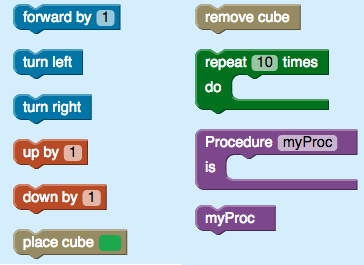
\includegraphics[width=\columnwidth]{images/toolbox-wide}
  \caption{The programming elements available in \gametitle{}.}
  \label{fig:toolbox}
\end{figure}


\section{Research Questions}
\label{sec:research}

Our primary goal for \gametitle{} is to investigate questions in computer science education and game-based learning. 
Specially, we are interested in exploring how to teach computational thinking skills and problem-solving strategies, and we are interested in exploring which programming languages best support novices in learning these skills. 
This naturally leads to research questions on how an effective educational game should be structured.
Open-ended games and systems typically perform poorly at teaching complex concepts without instructors or other outside help, but linear, direct-guidance based games and systems don't offer the engaging creative and social experiences that can be found in more open-ended settings.
In this section, we describe these research problems in detail and design decisions informed by these problems.

\subsection{Teaching Computer Science}

\subsubsection{Compuational Thinking}

% what is it
A major goal of our project is to explore methods of teaching \emph{computational thinking}~\cite{wing2008computational} skills.
Many have studied how to increase presence and effectiveness of computational thinking in computer science education (and education in general)~\cite{barr2011bringing, lye2014review},
while others have developed games to teach these ideas~\cite{weintrop2013robobuilder, kazimoglu2012serious}. 
Repenning et al.~\cite{repenning2010scalable} suggest six properties a computational thinking tool for K-12 must have in order to achieve systemic impact. 
Evaluating and characterizing the effectiveness of systems that use these (and other) properties is an ongoing research effort.

\gametitle{}'s design is structured to encourage and require use of computational thinking skills.
Like many programming games, we force the player to automate tasks that they are used to performing manually (in this case, the construction of 3D block structures).
As the player sets more sophisticated goals, abstraction becomes important (e.g., abstracting the building of a wall into a procedure) to keep the visual programming feasible. 

% how can we teach it directly?
As we cannot expect players to learn such complex and abstract skills simply by playing in an environment that requires them, we explore how to effectively directly teach computational thinking skills.
One such skill is a core component of computational thinking: the identification and application of problem-solving strategies such as divide and conquer.
A great deal of recent education research suggests that ``curricula can model such strategies for students'' and that appropriate guidance, which in many cases consists of the capabilities afforded by a suitable computational environment, can ``enable students to learn to use these strategies independently''~\cite{report2010computational}.
Mayer and Wittrock call attention to the substantial evidence in the education literature for teaching what they call \emph{domain-specific thinking skills} and \emph{metacognitive skills}~\cite{mayer1996handbook}.
The former would include the ability to use a strategy like divide and conquer, and the latter would include knowing when and where to employ that strategy.
In both cases, Mayer and Wittrock describe studies (for non-computer science domains) that have shown teaching these skills directly can improve learning and performance, and it is an open question whether this can be applied to teaching computational thinking in a game.

% teaching stategies like divide and conquer
Our initial attempt to directly teach divide-and-conquer is to lead the player though a top-down deconstruction of building a large castle.
The player is presented with a single code block that builds an entire castle, but discovers the construction has a number of flaws. 
The next several puzzles each decompose some part of the flawed program in order to give the player a chance to repair it. 
For example, to enable the player to give the castle the correct number of walls and towers, the castle code block is split into a tower block and a wall block that the player uses to write a corrected castle procedure, as shown Figure~\ref{fig:decomp}. 
This part of \gametitle{} needs to be expanded and refined before it can be evaluated, but the larger question certainly merits further attention. 

\begin{figure*}[th!]
  \centering
  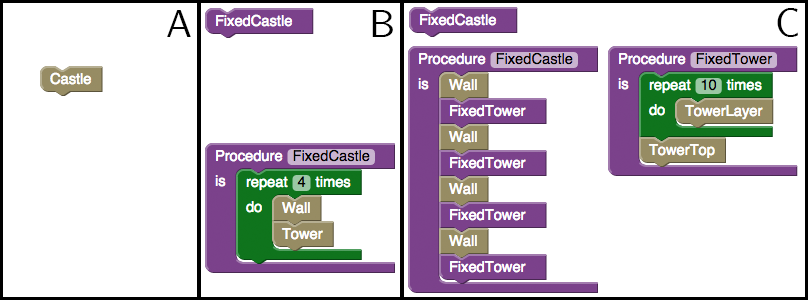
\includegraphics[width=\textwidth]{images/decomp-code}
  \caption{The code required by a progression of levels demonstrating the strategy of divide and conquer. In A, the player uses a single code block to build an entire castle. Then, in B, the player is given an empty \texttt{FixedCastle} procedure, which they must fill with the appropriate number of wall and tower blocks. Finally, in C, the player is given a completed \texttt{FixedCastle} procedure and must fill in the \texttt{FixedTower} procedure as shown. The final completed castle is shown on the right.}
  \label{fig:decomp}
\end{figure*}

\subsubsection{Language Semantics for Novices}

For those just starting to program, many aspects of the programming language and programming environment can affect their progress. 
Language syntax and semantics have been extensively studied for professional programmers~\cite{hudak1994haskell, kennedy2004defining, delorey2007programming}.
Previous work on programming for novices indicates aspects such as language syntax~\cite{stefik2013syntax}, compiler messages~\cite{nienaltowski2008compiler}, and language semantics~\cite{hoc1990language} can all have an impact, but only syntax and compiler messages have been characterized in detail. 
So while we can draw on existing research when choosing the programming syntax and input method, it an open problem which language semantics help novices learn programming and computational thinking.


\gametitle{} uses a custom visual programming language instead of using a popular existing language like JavaScript, which comes with several benefits and problems.
The primary benefit of the approach is that we have fine-grained control over language semantics, enabling future experimentation and comparative studies on language semantics.
However, this comes with several downsides over using an existing language.
The most apparent drawback of this approach is the lack of existing resources for students to use.
Using an existing popular language not only comes with a very large and free corpus of learning material, but provides an avenue for students to apply what they have learned directly outside the game.
On the other hand, choosing an existing language requires inheriting and quirks of that language.
Finally, some visual programming tools, such as Code.org, offer conversion to the equivalent concrete syntax.
With a general-purpose language, this transformation is 1-way only, since many syntactic constructs cannot be expression in the visual language.

%Finally, we have implemented a concrete syntax for our language that corresponds precisely with its visual code-block equivalent, allowing translation to and from concrete syntax, allowing players to choose which method of input they prefer.  

\subsection{Structure of Learning Environment}

\subsubsection{Guided Discovery Learning}
\label{sec:guided_discovery_theory}

Teaching complex skills such as computational thinking or programming though interactive software is very challenging, and any effort to do so in a game naturally leads to research questions about which structures are most effective.
For example, some games are structured as a sandbox where players discover the properties of the environment through largely unguided exploration (e.g., \emph{Minecraft}, \emph{SimCity}~\cite{simcity}), while others provide a linear sequence of levels designed to teach the player the relevant information (e.g., \emph{Portal}~\cite{portal}). 

In terms of learning theory, the former is known as \emph{discovery learning}, in which learning takes place through exploration with the object of study.
A major advantage it can have over a traditional teaching approach is motivational: directly exploring and interacting with something can be substantially more engaging than hearing someone talk about it.
Furthermore, this allows learning domains to be grounded in an application of interest to the learner, creating meaning and intrinsic interest in developing the desired skills.
While the pure form of this approach can work for simple learning domains, complex ones such as programming or computational thinking cannot be taught through exploration alone unless players have sufficient background knowledge~\cite{kirschner2006minimal}. 

The recommended practice is for systems to use \emph{guided discovery}, in which discovery learning is paired with some kind of external direct guidance~\cite{mayer2004should}.  For example, in games, players might consult wikis or ask friends to help them develop high-level skills.
This approach of combining settings for discovery learning with guidance is a central part of \emph{constructionism}, a learning theory that proposes students learn effectively by constructing things of social relevance in a social context~\cite{kafai06constructionism}.
Scratch~\cite{maloney2010scratch}, which enables users to create interactive digital media projects such as stories and games, is among the most popular of systems designed with constructionist principles.
Scratch's open-ended creative environment allows player to pursue meaningful creative projects, giving them motivation to learn the programming skills required to do so.
However, the tool in isolation cannot effectively teach these skills.
It is designed such that the social community or possibly instructors and mentors help teach new users.

On the other hand, more structured systems can more effectively teach skills without external guidance by limiting player freedom.
Linear games such as \emph{Portal} introduce concepts in a deliberate ordering and pacing to allow players to develop skills.
Methods of direct instruction also fall into this category, such as standard classroom lectures.
Online systems such as Code.org pair linear sequences of puzzles with videos to explain and teach the concepts.

Other games teach players by doing something in between. 
Games in the Zelda series (e.g., \emph{The Legend of Zelda: Ocarina of Time}~\cite{zelda_oot}) contain a non-linear sequence of puzzles and teach new mechanics by requiring the player demonstrate understanding of a new mechanic before they are allowed to progress. 
Strategy games such as \emph{Crusader Kings II}~\cite{ck2} offer a set of explicit tutorials the player may choose to go through before beginning more open-ended play.

Both types of systems (open-ended vs.\ highly-structured) have highly desirable benefits.
The open research problem we have begun exploring is how to create a hybrid model that best combines benefits of both approaches, particularly in settings where we cannot rely on an instructor.
Our initial approach joins an open sandbox with voluntary small sequences of puzzles that directly guide players.
Our playtesting has shown this to be a promising, though this encounters several design challenges. We discuss associated trade-offs in Section~\ref{sec:direct_guidance}.
The primary challenge with direct guidance in an open-ended game is providing guidance at the appropriate moment;
effective games provide help on-demand and just-in-time~\cite{gee2003video}.

\subsubsection{Social Environments}
\label{sec:social}

An effective technique for providing guidance and guided discovery is through social environments.
Social communities both create motivation to learn (to impress the social group) and guidance (by getting help from the group).
\emph{Scratch} users, for example, have shared millions of projects and even formed online companies to tackle projects together~\cite{resnick2009scratch}. 
Research using an online programming environment called MOOSE Crossing~\cite{bruckman1997moose} found that a social context can support and motivate learning programming~\cite{bruckman2000situated}.
This work is supported by research in behavioral and social sciences that indicates sharing and collaboration can improve learning~\cite{bransford2000people}. 

Social environments are also a critical aspect of learning in many games, including non-educational games.
The communities surrounding skill-based games (wikis, forums, conferences) help players learn effective high-level skills and strategies~\TODO{cite, someone definitely looked at this}.
Open-world multiplayer games, notably \emph{Mincraft}, have been used effectively as a virtual classroom environment~\TODO{cite}.
Players working together in \emph{Minecraft} are able to share their work, collaborate with others, and help directly guide others.

We have so far incorporated the project-sharing features of \emph{Scratch}.
A player can choose to share anything they build in the sandbox, sending it to a gallery containing everyone's shared creations.
Browsing the gallery, players can view, and get the code for, any uploaded construction.
However, a much more desirable goal is support close collaboration like pair programming or a \emph{Minecraft}-like shared world.
This encounters several design challenges, which we describe in Section~\ref{sec:multiplayer}.

\section{Open Design Problems}
\gametitle{}'s design and research goals have led to several tensions and difficulties.
In this section we discuss cases where the gaols have presented unusual challenges, and relevant results from pilot tests.

\subsection{Guided Learning in a Sandbox}
\label{sec:direct_guidance}

Section~\ref{sec:guided_discovery_theory} introduced \emph{guided discovery learning} and the techniques games and educational systems use to approach teaching.
In \gametitle{}, our difficult design goal is to center the experience in an open sandbox (like, e.g., \emph{Minecraft}) but provide on-demand, just-in-time direct guidance for new tools and concepts in the form of small puzzle segments.

The ideal we are trying to emulate, like much educational software, is a personal human tutor.
An effective tutor can allow the player to explore in the sandbox, and, once the player expresses the need for a tool or feature they do not yet possess, the tutor can guide them to the appropriate learning material.
Knowing when to intervene and what the player is trying to do is a challenge.
Intelligent tutoring systems accomplish this by tracking player knowledge and skill, which requires both a model of all conceptual knowledge and a rigid structure of problems with known solution strategies.
As we have neither of these, this is not an option.

The game must strike a difficult balance: get the player to the sandbox where they can experiment as quickly and often as possible, but support the player in the gradual acquisition of new knowledge and skills. 

We do not wish to overwhelm new players with the full suite of features and tools upon start, so they are locked behind puzzles until the player has a chance to learn about them in a guided, isolated setting.
Puzzle sequences need to be relatively short to minimize frustration and boredom; they should give players the knowledge they need and allow them to return to the sandbox.
Once unlocked, players have free use of tools in the sandbox.
A list of available learning modules advertise what techniques and tools players can gain from puzzles.
This is in tension with the desire to quickly allow a player access to the tools they need without jumping through hoops and challenges. 
Systems like \emph{Scratch} are fully open from the start, and expect an expert to guide newcomers through the system.

Even if committed to the design of gated introduction of features, there are difficult questions about what should be unlockable when.
The total set of features and strategies available are quite large, and freedom to learn \emph{all} of them immediately may overwhelm players.
Content is instead currently arranged into a graph, where prerequisite concepts must be unlocked before access to more complex ones is granted.
This, however, makes it difficult for players to determine if a feature is completely absent or if they simply have not unlocked it yet.

Empirically, players initially struggle with the structure but enjoy it once it is explained to them.
Very few players discover the puzzles without external guidance, a clear failure point if we wish the system to function without an instructor.
In playtests, players would often ask if they game supports a feature (e.g., moving up and down, removing blocks), when such a feature was directly advertised in the list of available modules.
After being informed of this, players began to understand the basic loop and would check for other skills they could learn through puzzles.

Other players can also be a source of guidance and ideas, so the social features will play an important role in this process.
For example, a friend in \emph{Minecraft} can jump-start a new player by giving them tools and showing them around.
Perhaps, in our game, veteran players could unlock tools for new players to let them bypass the built-in gating when mentoring them.

We have also found that creating in the sandbox is not necessarily the activity of choice for every player. 
Some choose to doodle in the sandbox, scattering cubes, often of different colors, in lines and clusters without trying to assemble anything in particular.
Others exclusively seek out the game's puzzles, more interesting in solving those than working in the sandbox.
Theoretically, this game structure should allow \gametitle{} to appeal to players with either interests, though it currently requires both parts.

\subsection{Collaboration in a Multiplayer\\Environment}
\label{sec:multiplayer}

As discussed in Section~\ref{sec:social}, social environments are an important part of guiding discovery learning and a major goal of our project.
The goal is to create a shared virtual environment in which players can assist each other and collaborate.
This works naturally in multiplayer games such as \emph{Minecraft}, where players on the same game server can explore and shape a persistent world together.
This shared world has several benefits.
It is easy for players to share their creations with others, but at the same time work relatively independently.
Changes to the world are localized around the player, so one player does not interfere with those far away.
At the same time, working closely together is as simple as walking to the same place in the world, where players can assist each other.

Such interactions could be invaluable for programming, supporting activities such as pair programming and mentoring of new concepts.
However, the persistent world model conflicts with other design considerations.
It is very easy to accidentally (or intentionally) write programs that have non-localized effects, interfering with others in the shared world.
Programming often relies on rerunning the same program over and over to iterate and find bugs, but this requires resetting the world state to a consistent start state.
While such a reset or undo feature is an option, if a player writes code the places blocks all over another player's work, how should the game reset state in a consistent and understandable manner?
This tension is even present without the multiplayer setting.
Playtesters that wanted to construct complex objects, such as a town of buildings, often wanted to do so piecemeal. They write separate programs to build each part without wanting to reset the world to a start state.

Our current approach does not sufficiently resolve this tension, and only addresses the single-player setting.
The sandbox makes the effects of programs permanent by default, including any cubes placed and the dragon's position.
To allow for experimentation, the player has the option to switch to \emph{workshop mode}, which resets the world to its previous state each time the player runs a new program. 
The player can freely toggle between these two modes, testing out each program before committing to its results. 
In practice, players have a difficult time understanding the nuanced difference between the two modes, despite dramatic visual cues.
The feature is empirically both difficult to discover and difficult to understand even once explained.

\section{Related Work}

\subsection{Educational Technology and Games\\for Computer Science}

The development of tools designed to teach novices programming dates back to systems such as Pappert's LOGO~\cite{papert80mindstorms}.
Kelleher and Pausch review programming environments for novices and describe a taxonomy of these systems~\cite{kelleher2005lowering}.
Within that taxonomy, \gametitle{} fist best as a teaching system that targets \emph{structuring programs} and aims to provide learning support both through \emph{social learning} and \emph{providing a motivating context}. 
In this section, we summarize the current space of educational programming tools. 
We separate them into two broad categories according to their structure: open-ended, largely unstructured systems that allow users to creatively explore and systems that present users with a linear sequence of problems or puzzles to solve. 

\subsubsection{Open-Ended Creative Systems}
Both early tools like LOGO and recent tools like \emph{Scratch} have an open-ended and creative approach.
LOGO allowed players to create drawings by controlling a robot with a virtual pen.
While LOGO was text-based, many modern examples use visual programming languages. 
\emph{Alice}~\cite{cooper2000alice}, like \emph{Scratch}, focuses on storytelling, though it does so in a 3D animation context with more fine-grained control than Scratch offers.
Other systems such as \emph{AgentSheets}~\cite{repenning2000agentsheets} and \emph{Kodu}~\cite{kodu} let users create simulations and games.
\emph{AgentSheets} models its world as agents on a grid, and players can program the behavior of each type of agent, conditioning behavior on the contents of adjacent grid cells. 
Designed for the Xbox as well as PC, \emph{Kodu} users program the behavior of each entity by setting up a series of event triggers and corresponding actions. The large number of available triggers and actions are accessed through a series of menus. 

There are also educational programming games that have their players tackle open-ended challenges.
\emph{CodeSpells}~\cite{esper2013codespells} is a game in which players write Java code to cast spells that control their environment. 
In \emph{RoboBuilder}~\cite{weintrop2013robobuilder}, players program robots to battle against enemies.

\subsubsection{Structured Learning Systems}
Another type of programming educational system is instead arranged as a linear sequence of problems or puzzles.
Step-by-step lessons are available from Khan Academy~\cite{khanacademy} and Codecademy~\cite{codecademy}, in which users program in a popular industry programming language such as Javascript or Java, sometimes with accompanying video.
Code.org~\cite{codedotorg} is a sequence of videos and puzzles where users control characters from popular games like Rovio's \emph{Angry Birds} or movies like Disney's \emph{Frozen} with drag-and-drop programming (like \emph{Scratch}).

Some games also fall into this category.
The game \emph{LightBot}~\cite{lightbot} asks players to use programming to control a robot in a sequence of linear puzzles.
The game has been used to study education in computational thinking~\cite{Gouws13Lightbot}, and is now featured in Code.org's Hour of Code~\cite{lightbothoc}.
\emph{BOTS} is a programming puzzle game. The stated goal of the project is to study how community-authored content is used in educational games~\cite{hickspart14}, and it has also been used to explore hint generation~\cite{peddycord14generating}.
We wish to combine direct lessons and open-ended structure into a single system, and explore the trade-offs and whether we can get advantages from both types of systems.

Program By Design~\cite{programbydesign} is a curricula-oriented project that shares several principles with our approach, including gradually expanding the programming language. 
Following the course laid out in the textbook~\cite{felleisen2001design}, a student uses a series of subsets of the programming language Racket.
Like most computer science curricula, Program By Design gradually exposes the student to more programming concepts over time, but also prevents beginning students from dealing with unexplained language constructs or error messages depending on knowledge the student has not learned.
Adapting this curriculum, a related project called Bootstrap~\cite{bootstrap} uses videogame programming to teach algebra and geometry to middle school students.

\subsection{Related Learning Technologies}

\subsubsection{Intelligent Tutoring Systems}
Intelligent Tutoring Systems~\cite{koedinger06cognitive} have been successful applied to several teaching domains.
These tutors are typically rigidly structured, choosing which problem the student will work on next.
Some system employ results from cognitive psychology and thus are also called \emph{cognitive tutors}.
Techniques such as Knowledge Tracing~\cite{corbett1994knowledge} model student knowledge with a Bayesian framework.
This modeling requires experts to design a set of \emph{knowledge components} that encompass the skills and abilities players use, as well as a comprehensive set of production rules students use to solve problems in the tutor.

In \gametitle{}, we use direct teaching, but balanced with an open environment in an effort to make the experience more engaging and meaningful to players.
Projects such as \emph{Crystal Island} have integrated ITS technologies into educational games and found success with student knowledge modeling, goal recognition, and affect modeling~\cite{lester2013serious,rowe2010modeling}.
Student modeling is more challenging in games than rigid tutor environments, and this problem is even larger with open-ended games.
Creating a full set of production rules for an open-ended sandbox is not feasible since there are no direct goals.
Even with puzzle sections, creating the set of knowledge components is currently impractical for desired concepts such a meta-strategies for programming.

\subsubsection{Game-Based Learning}
Games have been steadily gaining attention as educational tools. 
Gee discusses games' potential for learning in a variety of subjects~\cite{gee2003video}.
He also describes ways \emph{good} games educate their players, including operating at the edge of a player's skill and allowing players to be producers as well as consumers.
A meta-analysis of research on games as educational tools found games can be effective in some educational settings, but require appropriate instructional support~\cite{ke2009qualitative}.
Such support could be external (provided by teacher facilitation, good team dynamics, or structured cooperative learning/playing) or internal (provided by debriefing, flexible scoring, progression of complexity, or other methods).

Games can be educational tools by design, or be adapted to educational purposes. 
\emph{Minecraft}'s popularity and its ability to engage children have prompted several efforts to use it as an educational tool.
\emph{MinecraftEdu}~\cite{minecraftedu} is an official variant of \emph{Minecraft} with a number of classroom-centric features. 
Teachers have used it in lessons on math, English, computer science, and other subjects.  
Zorn et al.\ created \emph{CodeBlocks}, a plugin for Minecraft that allows players to program a robot within the game, and they found that \emph{CodeBlocks} increased non-programmers' interest in programming~\cite{zorn2013minecraft}.
Another avenue people have tried is to teach programming by having students create modifications and plugins for \emph{Minecraft}, through mods such as \emph{ScriptCraft}~\cite{scriptcraft}.

\section{Conclusion}

Though the number of educational programming tools and the amount of research done with them has increased dramatically, systematic empirical work has remained sparse.
There are several under-explored research areas in computer science education and game-based learning, and we created \gametitle{} to investigate these questions.
These questions include how to teach problem-solving strategies such as divide-and-conquer and which language semantics are suitable for novices.
These directly lead to questions about the structure of the learning environment.
Fully open, discovery-learning approaches common to games and educational software require a teacher to be effective for complex learning domains like computational thinking.
We must explore the space between structured linear sequences and open-ended sandboxes without a teacher to guide.
Social settings play an important role in learning complex domains, but many details remained unresearched.

Players have so far responded positively to \gametitle{}, but several design challenges have arisen as a result of the research goals.
Balancing an open sandbox with direct-guidance puzzles proves challenging without a teacher to help students find appropriate puzzles.
Creating a collaborative shared environment clashes with the desire for the ability to reset and debug programs.
\TODO{final aspirational sentence?}

% Comment out in submission version
%\section{Acknowledgments}
%\TODO{copy from CHI papers?}

\bibliographystyle{abbrv}
\bibliography{ruthefjord-fdg-2015} 
\end{document}
